\documentclass[conference]{IEEEtran}
\IEEEoverridecommandlockouts

\usepackage{cite}
\usepackage{amsmath,amssymb,amsfonts}
\usepackage{graphicx}
\usepackage{textcomp}
\usepackage{xcolor}
\usepackage{booktabs}
\usepackage{tabularx}
\usepackage{url}
\usepackage{hyperref}

\hypersetup{
    colorlinks=true,
    linkcolor=black,
    citecolor=black,
    urlcolor=blue
}

\begin{document}

\title{Design and Development of a Five-Stage Pipelined RISC-V Processor Using Verilog HDL}

\author{
\IEEEauthorblockN{
\begin{tabular}{ccc}
\textbf{Yashkumar Nimje} & \textbf{Abhigya Sachdeva} & \textbf{Somraj Nandi} \\
\small GitHub: \texttt{WizardCarp85} & \small GitHub: \texttt{ABHIGYA0205} & \small GitHub: \texttt{somraj112} \\[8pt]
\end{tabular}
\\
\begin{tabular}{cc}
\textbf{Rudra Pratap Singh Choudhary} & \textbf{Saksham Narotra} \\
\small GitHub: \texttt{Rudra-choudhary} & \small GitHub: \texttt{sakshaaamm} \\[8pt]
\end{tabular}
}
\IEEEauthorblockA{
\textit{BTech, Modern Computer Architecture} \\
\textit{Rishihood University, Sonipat, Haryana}
}
}

\maketitle

\begin{abstract}
This project focuses on the design and modular development of a five-stage pipelined processor based on a subset of the RISC-V instruction set architecture (ISA), using Verilog hardware description language (HDL). The processor is organized into the Instruction Fetch (IF), Instruction Decode (ID), Execute (EX), Memory Access (MEM), and Write-Back (WB) stages. The architectural goal is to demonstrate how instruction processing can be divided into sequential stages so that different instructions may occupy different stages during the same clock cycle. Improved throughput is an architectural objective, not a measured result in the current project. The target instruction subset comprises \texttt{ADD}, \texttt{SUB}, \texttt{ADDI}, \texttt{LW}, \texttt{SW}, \texttt{BEQ}, and \texttt{BNE}. Relevant IF, ID, and EX components have been tested independently; complete end-to-end execution remains future work.

The design is developed using a modular approach, with separate Verilog modules for individual datapath components and pipeline registers. Simulation and functional verification are performed using Icarus Verilog, with GTKWave supporting optional Value Change Dump (VCD) waveform inspection. According to the current repository status, the Instruction Fetch, Instruction Decode, and Execute milestones have been implemented with unit and stage-level integration testbenches. The MEM and WB work assigned to M4, hazard-control completion and full top-level integration assigned to M5, and end-to-end performance evaluation remain subsequent development work. This report describes the architectural approach, implementation completed to date, verification strategy, current limitations, and planned extensions.
\end{abstract}

\begin{IEEEkeywords}
RISC-V, pipelined processor, Verilog HDL, Instruction Fetch, Instruction Decode, ALU, digital design, Icarus Verilog, GTKWave.
\end{IEEEkeywords}

\section{Introduction}
A processor executes machine instructions by performing arithmetic calculations, logical comparisons, memory reads, and memory writes. In a simple non-pipelined datapath, an instruction may use the processor's resources for several operations before the next instruction begins its execution. Pipelining divides instruction processing into stages. Once the pipeline is filled, multiple instructions can be processed concurrently, with each instruction occupying a different stage in a given clock cycle. Pipelining can improve instruction throughput, although the actual performance depends on stage delays, hazards, stalls, and other implementation details.

RISC-V is an open instruction set architecture designed around a reduced instruction set computing (RISC) approach. Its base instruction formats and modular design make it suitable for education, research, and hardware implementation. This project uses a limited subset of the RISC-V integer instruction set to focus on the fundamental operation of a processor rather than implementing the complete ISA.

\section{Literature Review}

\subsection{Reduced Instruction Set Computing (RISC)}
Reduced Instruction Set Computing relies on simplified, regular instruction formats and a load/store memory model to streamline hardware decoding and facilitate pipelined execution. Patterson and Ditzel established the foundational rationale for RISC architectures, highlighting how reduced instruction complexity directly decreases control logic overhead and improves execution regularity~\cite{b1}. 

\subsection{RISC-V Instruction Set Architecture}
The official RISC-V unprivileged architecture specification defines standard 32-bit base integer instruction encodings (RV32I), register conventions, immediate generation rules, and base integer semantics~\cite{b2}. While the broader RISC-V architecture supports variable-length instruction encodings (such as 16-bit compressed instructions), the base RV32I instructions implemented in this project are strictly 32-bit in width. These specifications provide the reference for the project's instruction decoder, immediate sign-extension logic, and main control unit. The architecture provides 32 general-purpose 32-bit registers, with register \texttt{x0} permanently hardwired to zero.

\subsection{Five-Stage Pipelined Organization and Hazard Mitigation}
Standard computer organization models divide instruction processing into five stages: Instruction Fetch (IF), Instruction Decode (ID), Execute (EX), Memory Access (MEM), and Write-Back (WB)~\cite{b3}. Pipeline registers preserve intermediate data and control signals across clock boundaries. However, pipelined execution introduces three primary classes of hazards: Data Hazards, Control Hazards, and Structural Hazards. Mitigating these requires data forwarding paths, pipeline stalls, and pipeline flushes. These techniques are planned parts of the later hazard-handling and integration work in this project.

\subsection{HDL Simulation and Waveform Analysis}
Hardware description languages such as Verilog allow digital systems to be modeled at the behavioral and register-transfer levels. Open-source verification workflows rely on Icarus Verilog (\texttt{iverilog} and \texttt{vvp}) to compile and execute self-checking testbenches, paired with GTKWave to inspect Value Change Dump (VCD) timing waveforms~\cite{b4,b5}. Simulation results should be recorded from actual test runs and should not be inferred from the existence of a testbench alone.

\section{Proposed Solution}

\subsection{Overall Five-Stage Pipeline Architecture}
The proposed processor partitions the datapath into five sequential stages separated by four synchronous pipeline registers (\texttt{IF/ID}, \texttt{ID/EX}, \texttt{EX/MEM}, and \texttt{MEM/WB}). Table~\ref{tab:isa} summarizes the target instruction subset.

\begin{figure*}[!t]
\centering
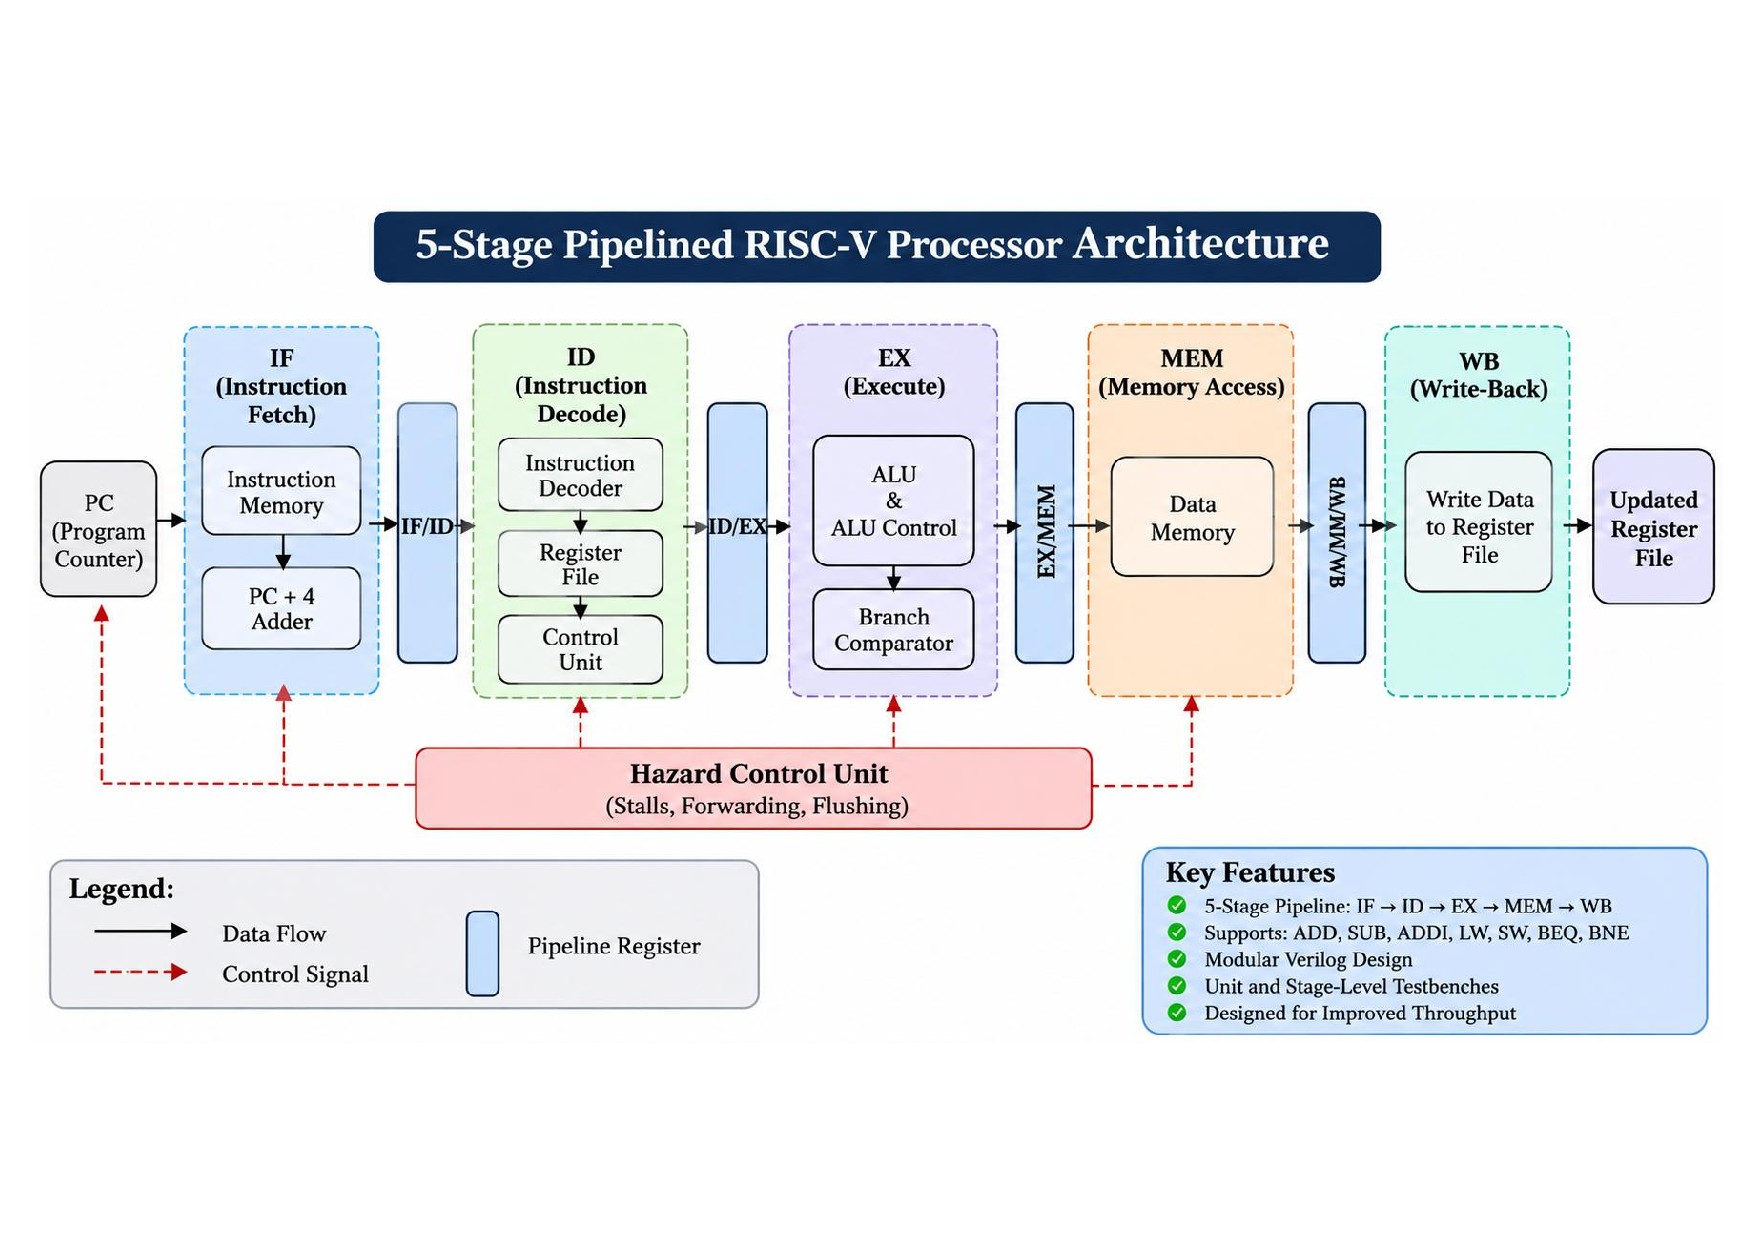
\includegraphics[width=\textwidth]{figures/pipeline_architecture_corrected.pdf}
\caption{Five-stage pipelined RV32I processor architecture and implementation status, illustrating verified stages (IF, ID, EX) with pipeline registers and operand forwarding paths alongside planned stages (MEM, WB) and hazard-integration logic.}
\label{fig:architecture}
\end{figure*}

\begin{table}[htbp]
\caption{Target RISC-V Instruction Subset}
\label{tab:isa}
\centering
\begin{tabularx}{\columnwidth}{@{}llX@{}}
\toprule
\textbf{Instr.} & \textbf{Type} & \textbf{Intended Datapath Operation} \\
\midrule
\texttt{ADD}  & R-type & Add two source register operands. \\
\texttt{SUB}  & R-type & Subtract the second register operand from the first. \\
\texttt{ADDI} & I-type & Add a 12-bit sign-extended immediate to a register. \\
\texttt{LW}   & I-type & Load a 32-bit word from data memory into a register. \\
\texttt{SW}   & S-type & Store a 32-bit word from a register to data memory. \\
\texttt{BEQ}  & B-type & Branch to target address when operands are equal. \\
\texttt{BNE}  & B-type & Branch to target address when operands are not equal. \\
\bottomrule
\end{tabularx}
\end{table}



\subsection{Instruction Fetch (IF) Stage}
The IF stage obtains an instruction from instruction memory using the program counter (PC). For sequential execution, the next instruction address is computed as $\text{PC} + 4$. The repository's IF implementation comprises:
\begin{itemize}
    \item \texttt{pc.v}: A 32-bit program counter with synchronous reset. It has no enable or stall input; a stall is intended to be achieved externally by feeding the current PC value back as \texttt{next\_pc}.
    \item \texttt{instr\_\allowbreak mem.v}: Instruction memory initialized from a hexadecimal program image using \texttt{\$readmemh}.
    \item \texttt{if\_\allowbreak stage.v}: A wrapper module integrating the PC and instruction memory to output the current PC, $\text{PC} + 4$, and fetched instruction.
    \item \texttt{if\_\allowbreak id\_\allowbreak reg.v}: A pipeline register capturing fetch outputs while supporting reset, flush, and hold behavior.
\end{itemize}

\subsection{Instruction Decode (ID) Stage}
The ID stage interprets the fetched instruction and prepares register operands, immediate values, and control signals:
\begin{itemize}
    \item \texttt{instruction\_\allowbreak decoder.v}: Extracts opcode, \texttt{rd}, \texttt{rs1}, \texttt{rs2}, \texttt{funct3}, \texttt{funct7}, and sign-extended immediate values.
    \item \texttt{register\_\allowbreak file.v}: Implements 32 general-purpose 32-bit registers with \texttt{x0} hardwired to zero and write-to-read bypass logic for simultaneous write-back and read of the same register.
    \item \texttt{main\_\allowbreak control.v}: Generates control signals for arithmetic, memory, branch, and register write-back behavior. 
    \item \texttt{id\_\allowbreak stage.v} and \texttt{id\_\allowbreak ex\_\allowbreak reg.v}: Structurally connect the decode components. The \texttt{uses\_rs1} and \texttt{uses\_rs2} source-operand usage indicators are generated by \texttt{id\_\allowbreak stage.v}, not by the main control unit.
\end{itemize}

\subsection{Execute (EX) Stage}
The EX stage executes arithmetic operations and evaluates conditional branches:
\begin{itemize}
    \item \texttt{alu.v}: A 32-bit arithmetic logic unit supporting \texttt{ADD} and \texttt{SUB} operations.
    \item \texttt{alu\_\allowbreak control.v}: Translates decoded ALU operation types and instruction function fields into ALU control codes.
    \item \texttt{branch\_\allowbreak unit.v}: Calculates branch target addresses and evaluates \texttt{BEQ} and \texttt{BNE} branch conditions.
    \item \texttt{ex\_\allowbreak stage.v}: Integrates the ALU, ALU control, branch unit, operand-selection multiplexers, and forwarding-input multiplexers.
    \item \texttt{ex\_\allowbreak mem\_\allowbreak reg.v}: Captures execution results, store data, destination register indices, and memory/write-back control signals.
\end{itemize}

\subsection{Memory Access (MEM), Write-Back (WB), and Hazard Control}
While the first three stages and their boundary registers are implemented in the current repository, the remaining stages represent planned development milestones:
\begin{itemize}
    \item \textbf{Memory Access (MEM) Stage:} Planned to perform data-memory reads for \texttt{LW} and writes for \texttt{SW} using the address calculated in the EX stage, followed by the \texttt{MEM/WB} pipeline register.
    \item \textbf{Write-Back (WB) Stage:} Planned to select between the data-memory output and the ALU result to write back into the destination register.
    \item \textbf{Hazard Control and Integration:} Planned to integrate hazard-detection logic for load-use stalls, forwarding-control generation for the EX-stage multiplexers, branch flush/redirect control, and top-level processor integration.
\end{itemize}



\section{Results and Discussion}
The design uses testbenches to verify individual modules and stage-level connections. The team recorded the observed output from the repository revision used for submission.

\begin{table}[htbp]
\caption{Testbench Simulation Results Summary}
\label{tab:results}
\centering
\begin{tabularx}{\columnwidth}{@{}lXl@{}}
\toprule
\textbf{Test} & \textbf{What it checks} & \textbf{Result} \\
\midrule
\texttt{tb\_alu} & \texttt{ADD}, \texttt{SUB}, flags, and unused operation codes & 80 checks passed \\
\addlinespace
\texttt{tb\_branch\_unit} & \texttt{BEQ}/\texttt{BNE} comparisons and branch-target calculation & 36 checks passed \\
\addlinespace
\texttt{tb\_ex\_stage} & EX datapath, operand selection, forwarding inputs, and control gating & 18 checks passed \\
\addlinespace
\texttt{tb\_ex\_mem\_reg} & Register capture, hold, flush, reset, and invalid/bubble behavior & 430 checked cycles \\
\bottomrule
\end{tabularx}
\end{table}

As reported in Table~\ref{tab:results}, \texttt{tb\_ex\_stage} performs 18 discrete test checks verifying combinational datapath correctness, operand selection, immediate multiplexing, forwarding inputs, and bubble side-effect suppression. In contrast, \texttt{tb\_ex\_mem\_reg} exercises 430 synchronous checked simulation cycles to comprehensively evaluate register capture, hold behavior, synchronous reset, pipeline flush, bubble handling, and a full 138-bit walking-bit pattern across the EX/MEM pipeline interface boundary.

At the current documented project stage, the IF, ID, and EX components and their associated pipeline registers have been implemented. The figures for \texttt{tb\_ex\_stage} and \texttt{tb\_ex\_mem\_reg} validate stage-level logic but do not represent full-CPU coverage or end-to-end execution. The complete five-stage processor is not yet documented as integrated. The MEM and WB datapaths assigned to M4, complete hazard-control logic and top-level integration assigned to M5, and end-to-end performance evaluation remain outstanding. Consequently, this report does not claim complete execution of all supported instructions through a fully integrated pipeline, nor does it claim a measured CPI or IPC result. 

\begin{table*}[!t]
\caption{Milestone Ownership and Individual Team Contributions}
\label{tab:contributions}
\centering
\begin{tabularx}{\textwidth}{@{}lllX@{}}
\toprule
\textbf{Contributor} & \textbf{GitHub Handle} & \textbf{Assigned Area} & \textbf{Technical Contributions and Scope} \\
\midrule
Yashkumar Nimje & \texttt{WizardCarp85} & M5 --- Hazard \& Integration & Established repository scaffold, contribution workflow (\texttt{CONTRIBUTING.md}), and PR templates; assigned to hazard-control completion and top-level processor integration (planned/in progress). \\
\addlinespace
Abhigya Sachdeva & \texttt{ABHIGYA0205} & M3 --- Execute Stage & Implemented \texttt{alu.v}, \texttt{alu\_\allowbreak control.v}, \texttt{branch\_\allowbreak unit.v}, \texttt{ex\_\allowbreak stage.v}, and \texttt{ex\_\allowbreak mem\_\allowbreak reg.v}; authored EX interface documentation and EX unit/stage testbenches. \\
\addlinespace
Somraj Nandi & \texttt{somraj112} & M2 --- Instruction Decode & Implemented \texttt{instruction\_\allowbreak decoder.v}, \texttt{register\_\allowbreak file.v}, \texttt{main\_\allowbreak control.v}, \texttt{id\_\allowbreak stage.v}, and \texttt{id\_\allowbreak ex\_\allowbreak reg.v}; authored ID interface documentation and ID unit/stage testbenches. \\
\addlinespace
Rudra Pratap Singh Choudhary & \texttt{Rudra-choudhary} & M4 --- Memory \& Write-Back & Assigned to the Memory and Write-Back milestone (data memory, MEM datapath, \texttt{MEM/WB} pipeline register, and WB selection path; currently planned/in progress) alongside repository reviews. \\
\addlinespace
Saksham Narotra & \texttt{sakshaaamm} & M1 --- Instruction Fetch & Implemented \texttt{pc.v}, \texttt{instr\_\allowbreak mem.v}, \texttt{if\_\allowbreak stage.v}, and \texttt{if\_\allowbreak id\_\allowbreak reg.v}; created the hexadecimal program image, IF interface documentation, and IF unit/stage testbenches. \\
\bottomrule
\end{tabularx}
\end{table*}

\section{Individual Contributions}
The project follows an issue-driven GitHub workflow using feature branches and pull-request reviews. Table~\ref{tab:contributions} details the milestone ownership across the team.



\section{Conclusion and Future Work}
This project documents the staged development of a five-stage pipelined RISC-V processor targeting a selected instruction subset. The current verified implementation status covers IF, ID, and EX components; complete end-to-end execution remains future work. The current implementation has established the first three stages. The IF stage includes the program counter, instruction memory, fetch wrapper, and IF/ID pipeline register. The ID stage includes instruction decoding, register-file access, control-signal generation, and the ID/EX pipeline register. The EX stage includes the ALU, ALU control, branch unit, execution datapath, and EX/MEM pipeline register. 

The project has therefore established a foundation for completing the memory and write-back datapaths and integrating the full pipeline. Icarus Verilog supports the simulation workflow, and GTKWave is available for waveform inspection when generated VCD files are examined. Future work includes completing the Memory Access and Write-Back stages, implementing the \texttt{MEM/WB} register, finalizing hazard-detection and forwarding control logic, integrating the top-level processor, and measuring end-to-end execution metrics such as CPI and IPC.

\begin{thebibliography}{00}
\bibitem{b1} D. A. Patterson and D. R. Ditzel, ``The Case for the Reduced Instruction Set Computer,'' \emph{ACM SIGARCH Computer Architecture News}, vol. 8, no. 6, pp. 25--33, Oct. 1980.
\bibitem{b2} A. Waterman and K. Asanovi\'{c}, Eds., \emph{The RISC-V Instruction Set Manual, Volume I: Unprivileged Architecture}, RISC-V International. [Online]. Available: \url{https://docs.riscv.org/reference/isa/unpriv/unpriv-index.html}
\bibitem{b3} D. A. Patterson and J. L. Hennessy, \emph{Computer Organization and Design RISC-V Edition: The Hardware/Software Interface}, 2nd ed. San Francisco, CA, USA: Morgan Kaufmann, 2020.
\bibitem{b4} S. Williams, \emph{Icarus Verilog}, Project Documentation and Source Repository. [Online]. Available: \url{https://github.com/steveicarus/iverilog}
\bibitem{b5} GTKWave Development Team, \emph{GTKWave}, Project Documentation and Source Repository. [Online]. Available: \url{https://github.com/gtkwave/gtkwave}
\end{thebibliography}

\end{document}